\chapter{A HLF Network for Healthcare} \label{HLFHealthcare} Altough many use
cases were presented in Section~\ref{background} they do not have the
technology that allows true private contracts and some of them use a currency
as a means to ensure the network consensus is achieved, by monetizing the
patients data.  After analyzing the different Blockchain implementations the
Fabric network was chosen as the foundation for this system. This
implementation was chosen to overcome previous works weaknesses and to match
the security and privacy that patients expect to have with their health data.
First we will discuss the tools provided to configure the network, and then
discuss the system architecture.

\section{Fabric Network Configuration Tools}

Hyperledger Fabric (HLF) does not use a centralized ledger where every record
is available to every participant in the network.  Instead it opts to allow
multiple ledgers in a network to achieve different goals of a greater purpose.
This allows the creation of channels of information between trusted parties,
for example, a channel of secure and private information between the clinical
staff of an hospital and a patient.

A HLF network is comprised by the \textit{cryptogen}, \textit{configtxgen},
\textit{configtxlator} and \textit{peer} tools that are used to configure the
network.

The \textit{cryptogen} tool generates cryptographic data consuming the file
\textit{crypto-config.yaml}.  HLF uses an abstraction layer for certification
and authority called Membership Service Provider (MSP) that defines the rules
by which entities are governed and authenticated and it must be unique for
every participating entity.

The \textit{configtxgen} tool generates the genesis block for the orderer
services and the initial transactions.  This tool consumes the file
\textit{configtx.yaml} that defines configuration parameters for channels, the
genesis block and the orderer service.

The \textit{configtxlator} tool is also used to generate channel configurations. 
Finally the \textit{peer} tool is used to manage the participating peers in the HLF network.

These tools are used to create and maintain the topology of the network and are
invoked when a change to the network is made, for example, when permissions to
certain records are changed or a new user is enrolled in the network and are
very much intertwined with the Certificate Authority (CA) server system to
maintain the security that is needed in a sensitive subject that deals with
private information.

\section{Identity Representation in Hyperledger}
 
HLF allows information to be written and read in a distributed manner with
security and privacy at the forefront. Using smart contracts, a record is
created to represent the concept of identity in this network.

The information that defines the patients identity is a key requirement to
build a system that recognizes patients across the Healthcare environment, as
discussed in Section~\ref{background}.  To this end, the identity of a patient
is recorded on the ledger of the HLF network as a structure via a smart
contract deployed to the network that interacts directly with the ledger.  This
structure contains the necessary fields to identify the patient such as its
name and birth date, for example, as well as some other information necessary
to manage this data. 

To aid in interoperability with other systems, as seen in Figure
\ref{fig:interoperability}, the Fast Healthcare Interoperability Resources
(FHIR) standard by the Health Level 7 organization was used as basis for the
representation of a patient.  Each field of the structure that represents the
patients identity, defined in the smart contract, is linked to a field of the
\href{http://www.hl7.org/fhir/patient.html}{patient structure as presented in
the FHIR standard}.

\begin{figure}[ht]
\centering
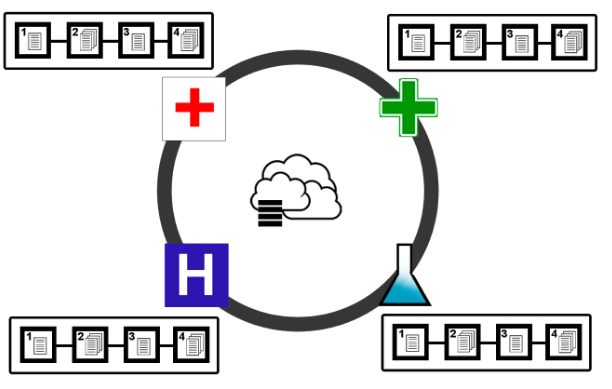
\includegraphics[width=0.7\linewidth]{imgs/interoperability.png}
\caption{\label{fig:interoperability}An Example of Interoperability with the Blockchain Network}
\end{figure}

\section{Application and Smart Contracts}

To create an interactive system that can manage the patients identity in an
Healthcare environment an application was built that the user interacts with.
This application interfaces with smart contracts through the Hyperledger Fabric
Software Development Kit and the chaincode was built using the Hyperledger
Fabric Shim for node.js.

The application is accessed by the user and calls upon the smart contract.  The
smart contract will handle the assets part of the system.  A smart contract to
represent and manipulate identity was built and interfaces with the network to
write and read records to the appropriate ledger. The overview of the
architecture for this system is represented on Figure \ref{fig:appOverview}.

\begin{figure}[ht]
\centering
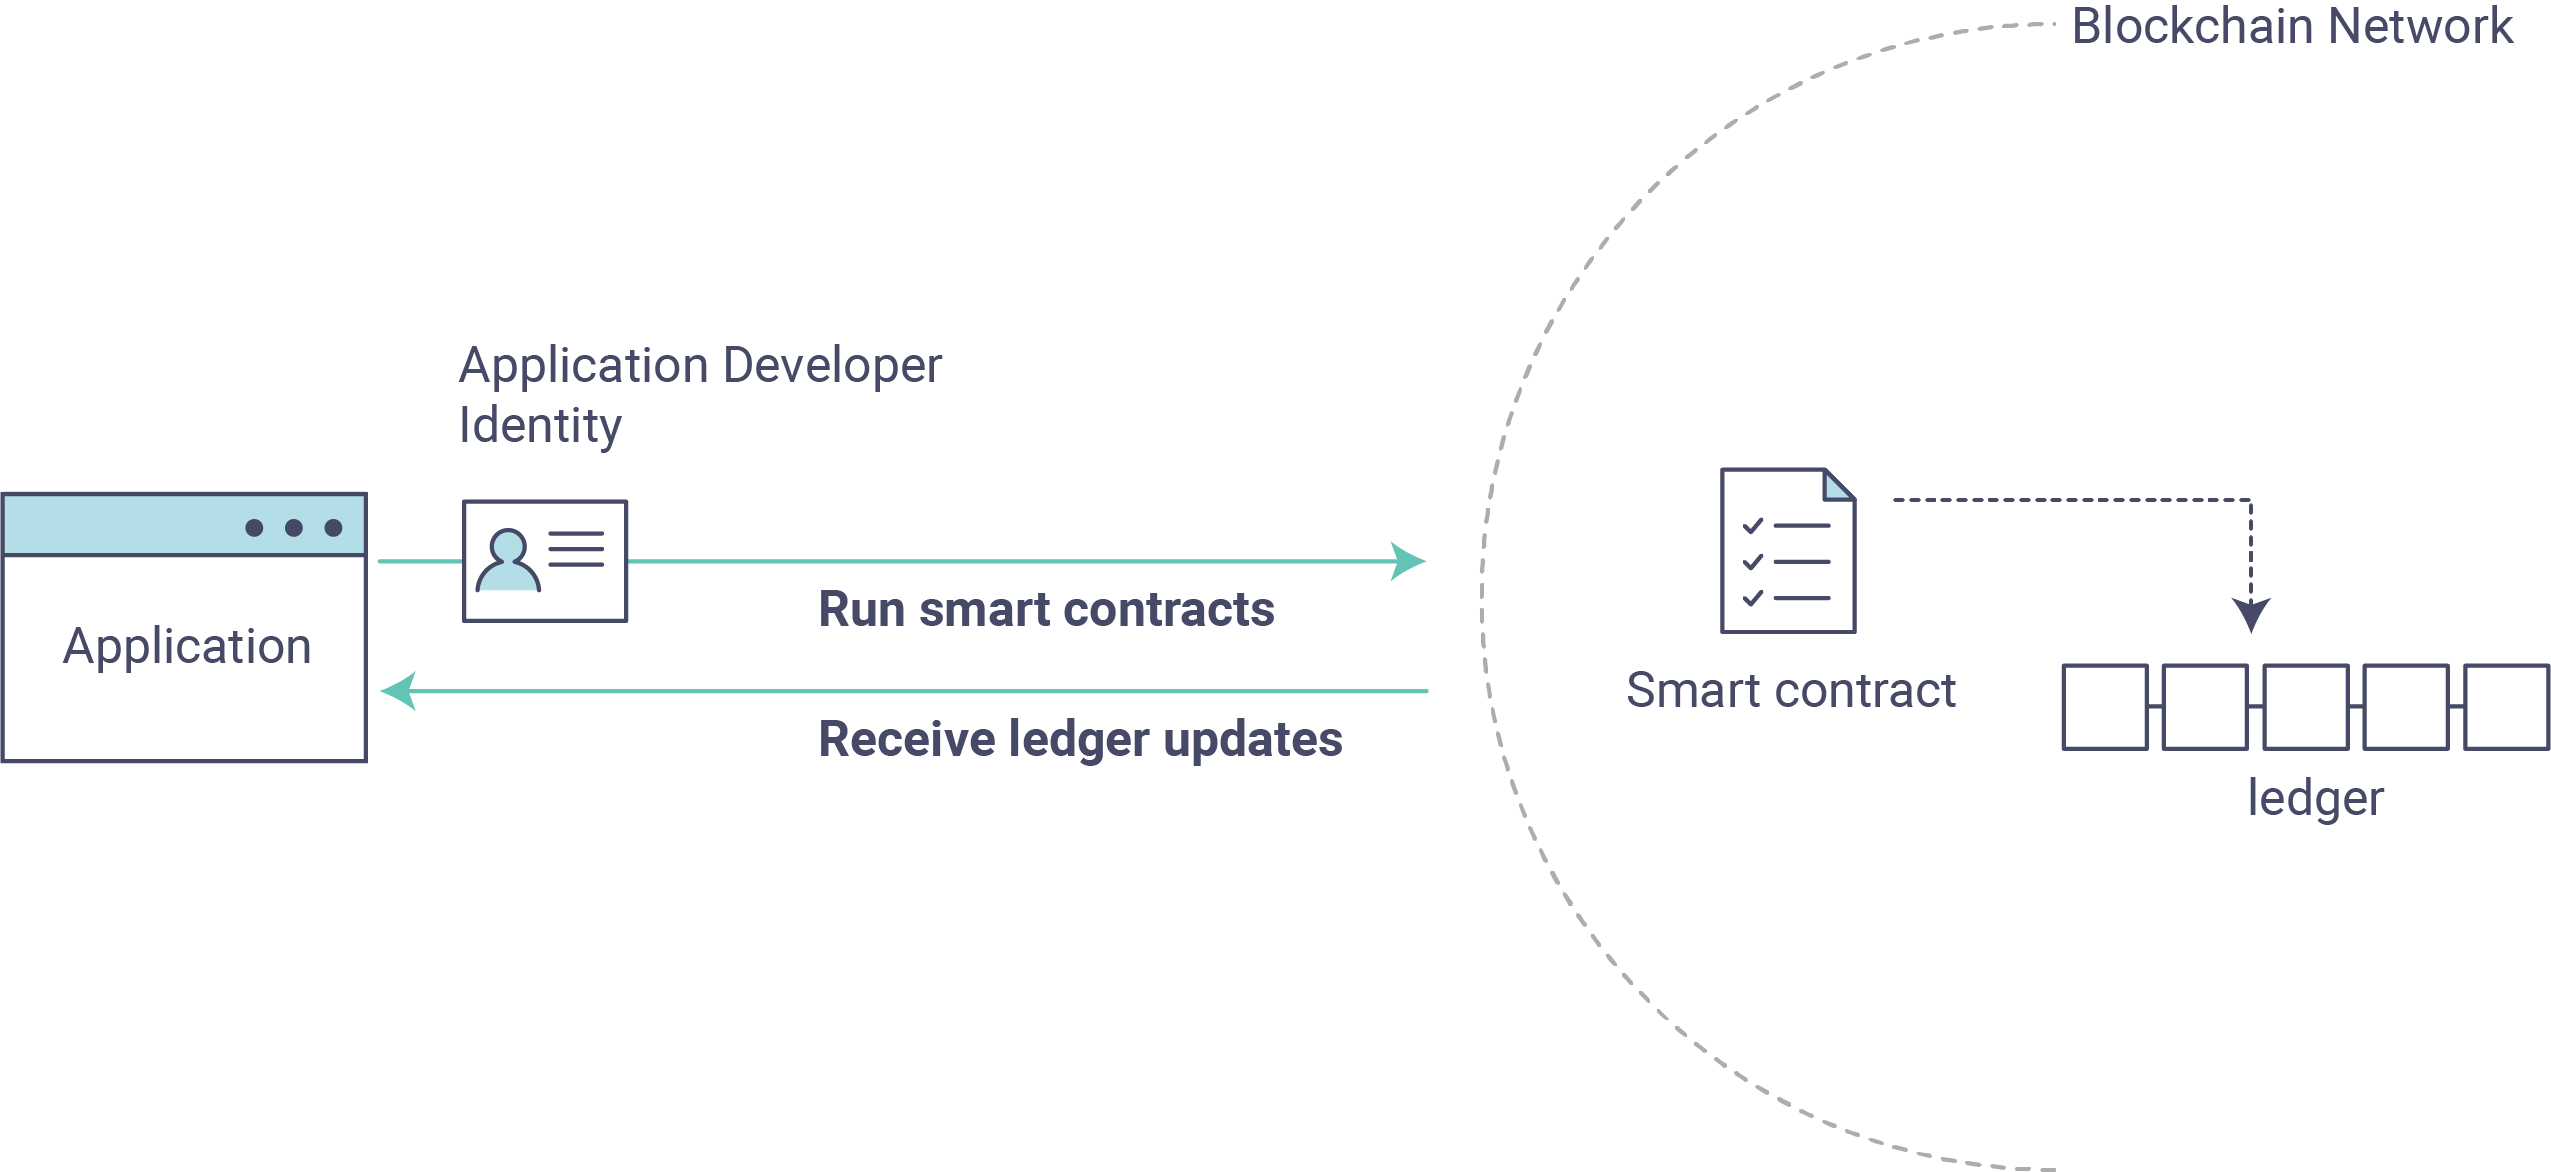
\includegraphics[width=1\linewidth]{imgs/hyperledgerAppOverview.png}
\caption{\label{fig:appOverview}An Overview of the System Architecture (Source: \href{http://hyperledger-fabric.readthedocs.io/en/latest/write_first_app.html}{HLF Fabric Documentation})}
\end{figure}

The application allows for user enrollment to create a new identity in the
network.  When a new user of the application enters the network; the function,
in the smart contract, that initializes the creation of the user and writes the
user to the ledger as a new participating identity is called. Due to the
security mechanisms this specific transaction is automatically signed by the
administrator of the network and is verified by the CA servers.

The smart contract also provides the application with several operations to
manage the identity object as seen on Figure \ref{fig:smartContractOverview}.
These operations form an Application Programming Interface (API) that return a
payload in JSON format with identity information from the network.  This API
allows a query to be made to the network that returns the patients information,
changing incorrect or outdated information or disabling the identity structure
of someone who is not participating in the network actively anymore in order
for that information to be read-only from that point on, for example, with more
available.  Depending on the operation only certain users can access the
information or manipulate the already existing one.  This system architecture
leads to a modular as well as extensible approach regarding the availability of
new operations that become available as soon as new versions of the smart
contract are deployed.  \begin{figure}[ht] \centering
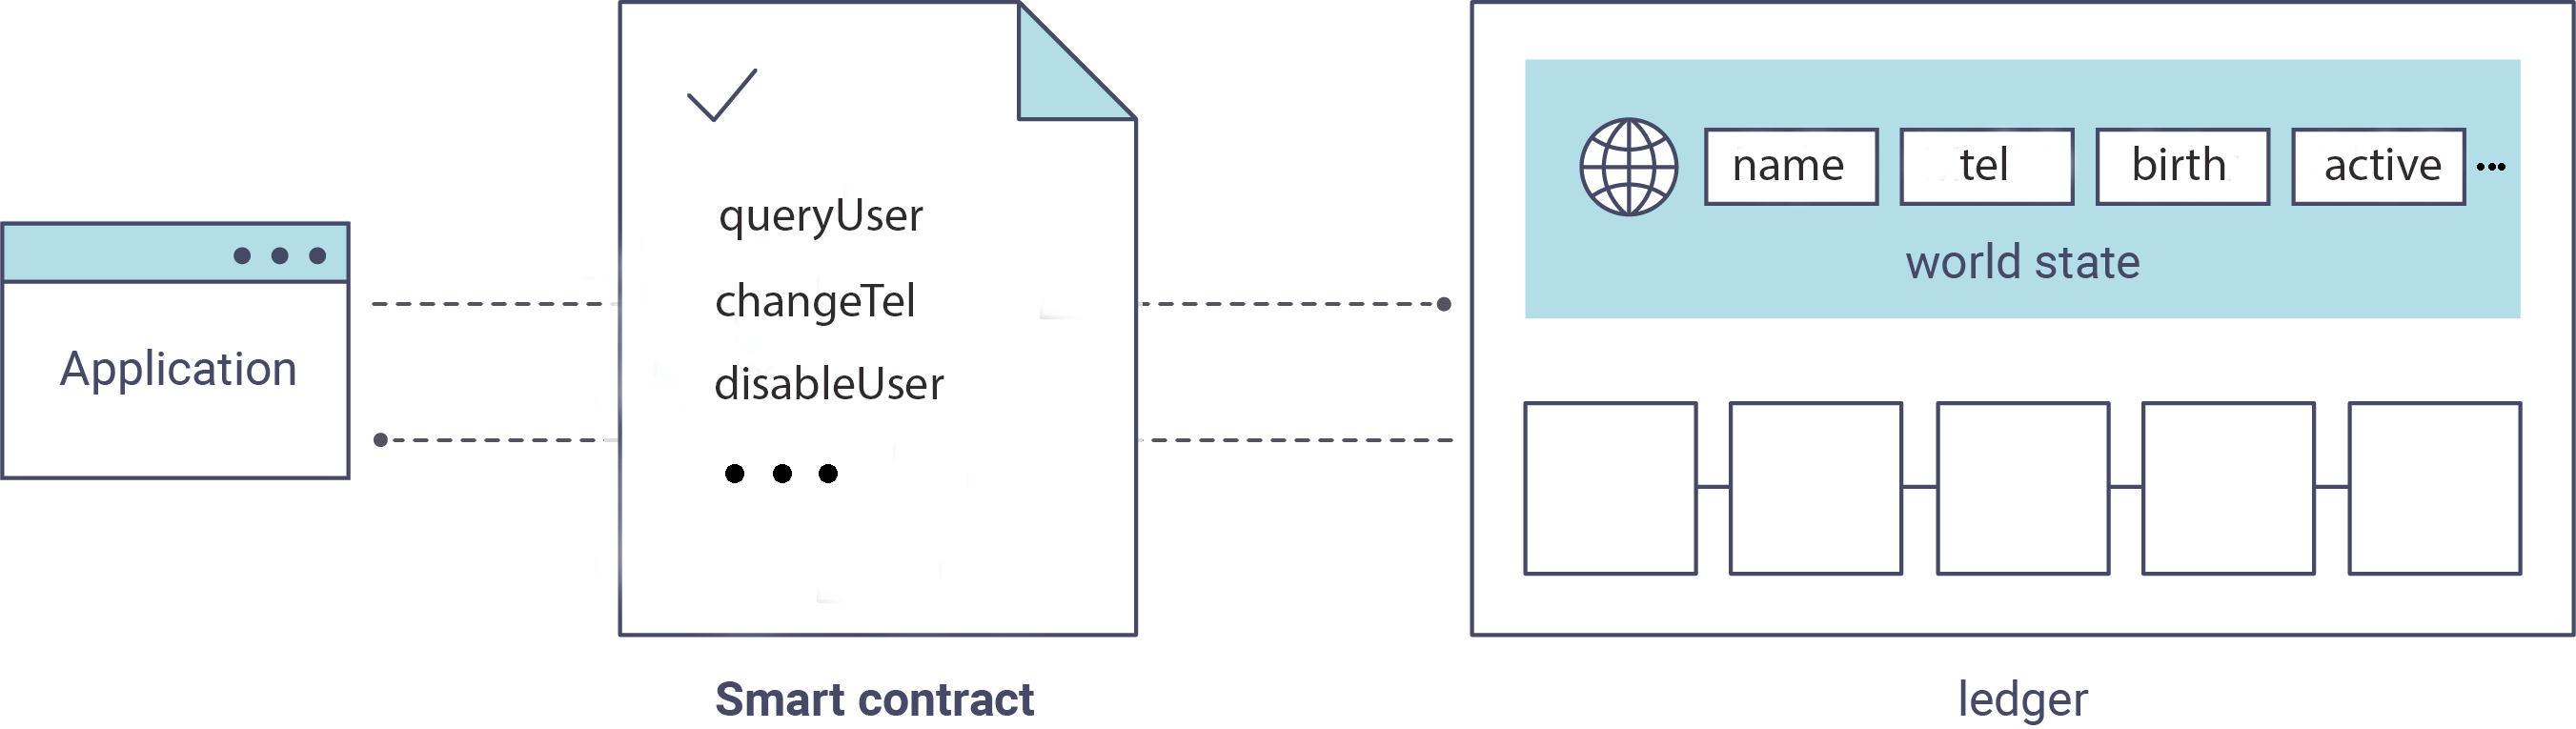
\includegraphics[width=1\linewidth]{imgs/smartContractOverview.png}
\caption{\label{fig:smartContractOverview}Smart Contract Operations Example
(Original:
\href{http://hyperledger-fabric.readthedocs.io/en/latest/write_first_app.html}{HLF
Fabric Documentation})} \end{figure}
